% Mini report: Pre-COVID productivity & lean user mechanisms
\documentclass{article}

% -------------------------------------------------------------------------
%  Packages (keep parity with consolidated‐report for tables)
% -------------------------------------------------------------------------
\usepackage{booktabs}
\usepackage{siunitx}
\usepackage{makecell}
\usepackage{threeparttable}
\usepackage{float}
\usepackage{amsfonts}
\usepackage{amssymb}
\usepackage{amsmath}
\usepackage{graphicx}  % figures
\usepackage[normalem]{ulem}
\usepackage{dsfont}
\usepackage{pdflscape}
\usepackage{tabularx}
\usepackage[colorlinks=true,linkcolor=blue,urlcolor=blue,citecolor=blue]{hyperref}

\usepackage{tabularx}
\usepackage[export]{adjustbox}
\usepackage{booktabs}


\usepackage{tabularx,array,booktabs,makecell,cellspace}
\renewcommand{\tabularxcolumn}[1]{m{#1}}
\setlength{\extrarowheight}{1.5pt}
\setlength\cellspacetoplimit{4pt}
\setlength\cellspacebottomlimit{4pt}

% define a “centering” version of X
\newcolumntype{C}{>{\centering\arraybackslash}X}

% Base directory for cleaned LaTeX tables
\newcommand{\cleanedresultsdir}{../../results/cleaned}
% Base directory for figures (shared with consolidated report)
% Figures are generated into the *project-root*/results/figures directory.
% Because pdflatex is invoked with -output-directory=build, we need to go up
% two levels to reach the repo root from writeup/build.
\newcommand{\figdir}{../../results/figures}

\begin{document}

% -------------------------------------------------------------------------
%  Table of contents (suppress automatic \clearpage inside)
% -------------------------------------------------------------------------


% -------------------------------------------------------------------------
%  Figures – key descriptive plots (replicated from consolidated report)
% -------------------------------------------------------------------------
\section{Figures}

\begin{figure}[H]
  \centering
  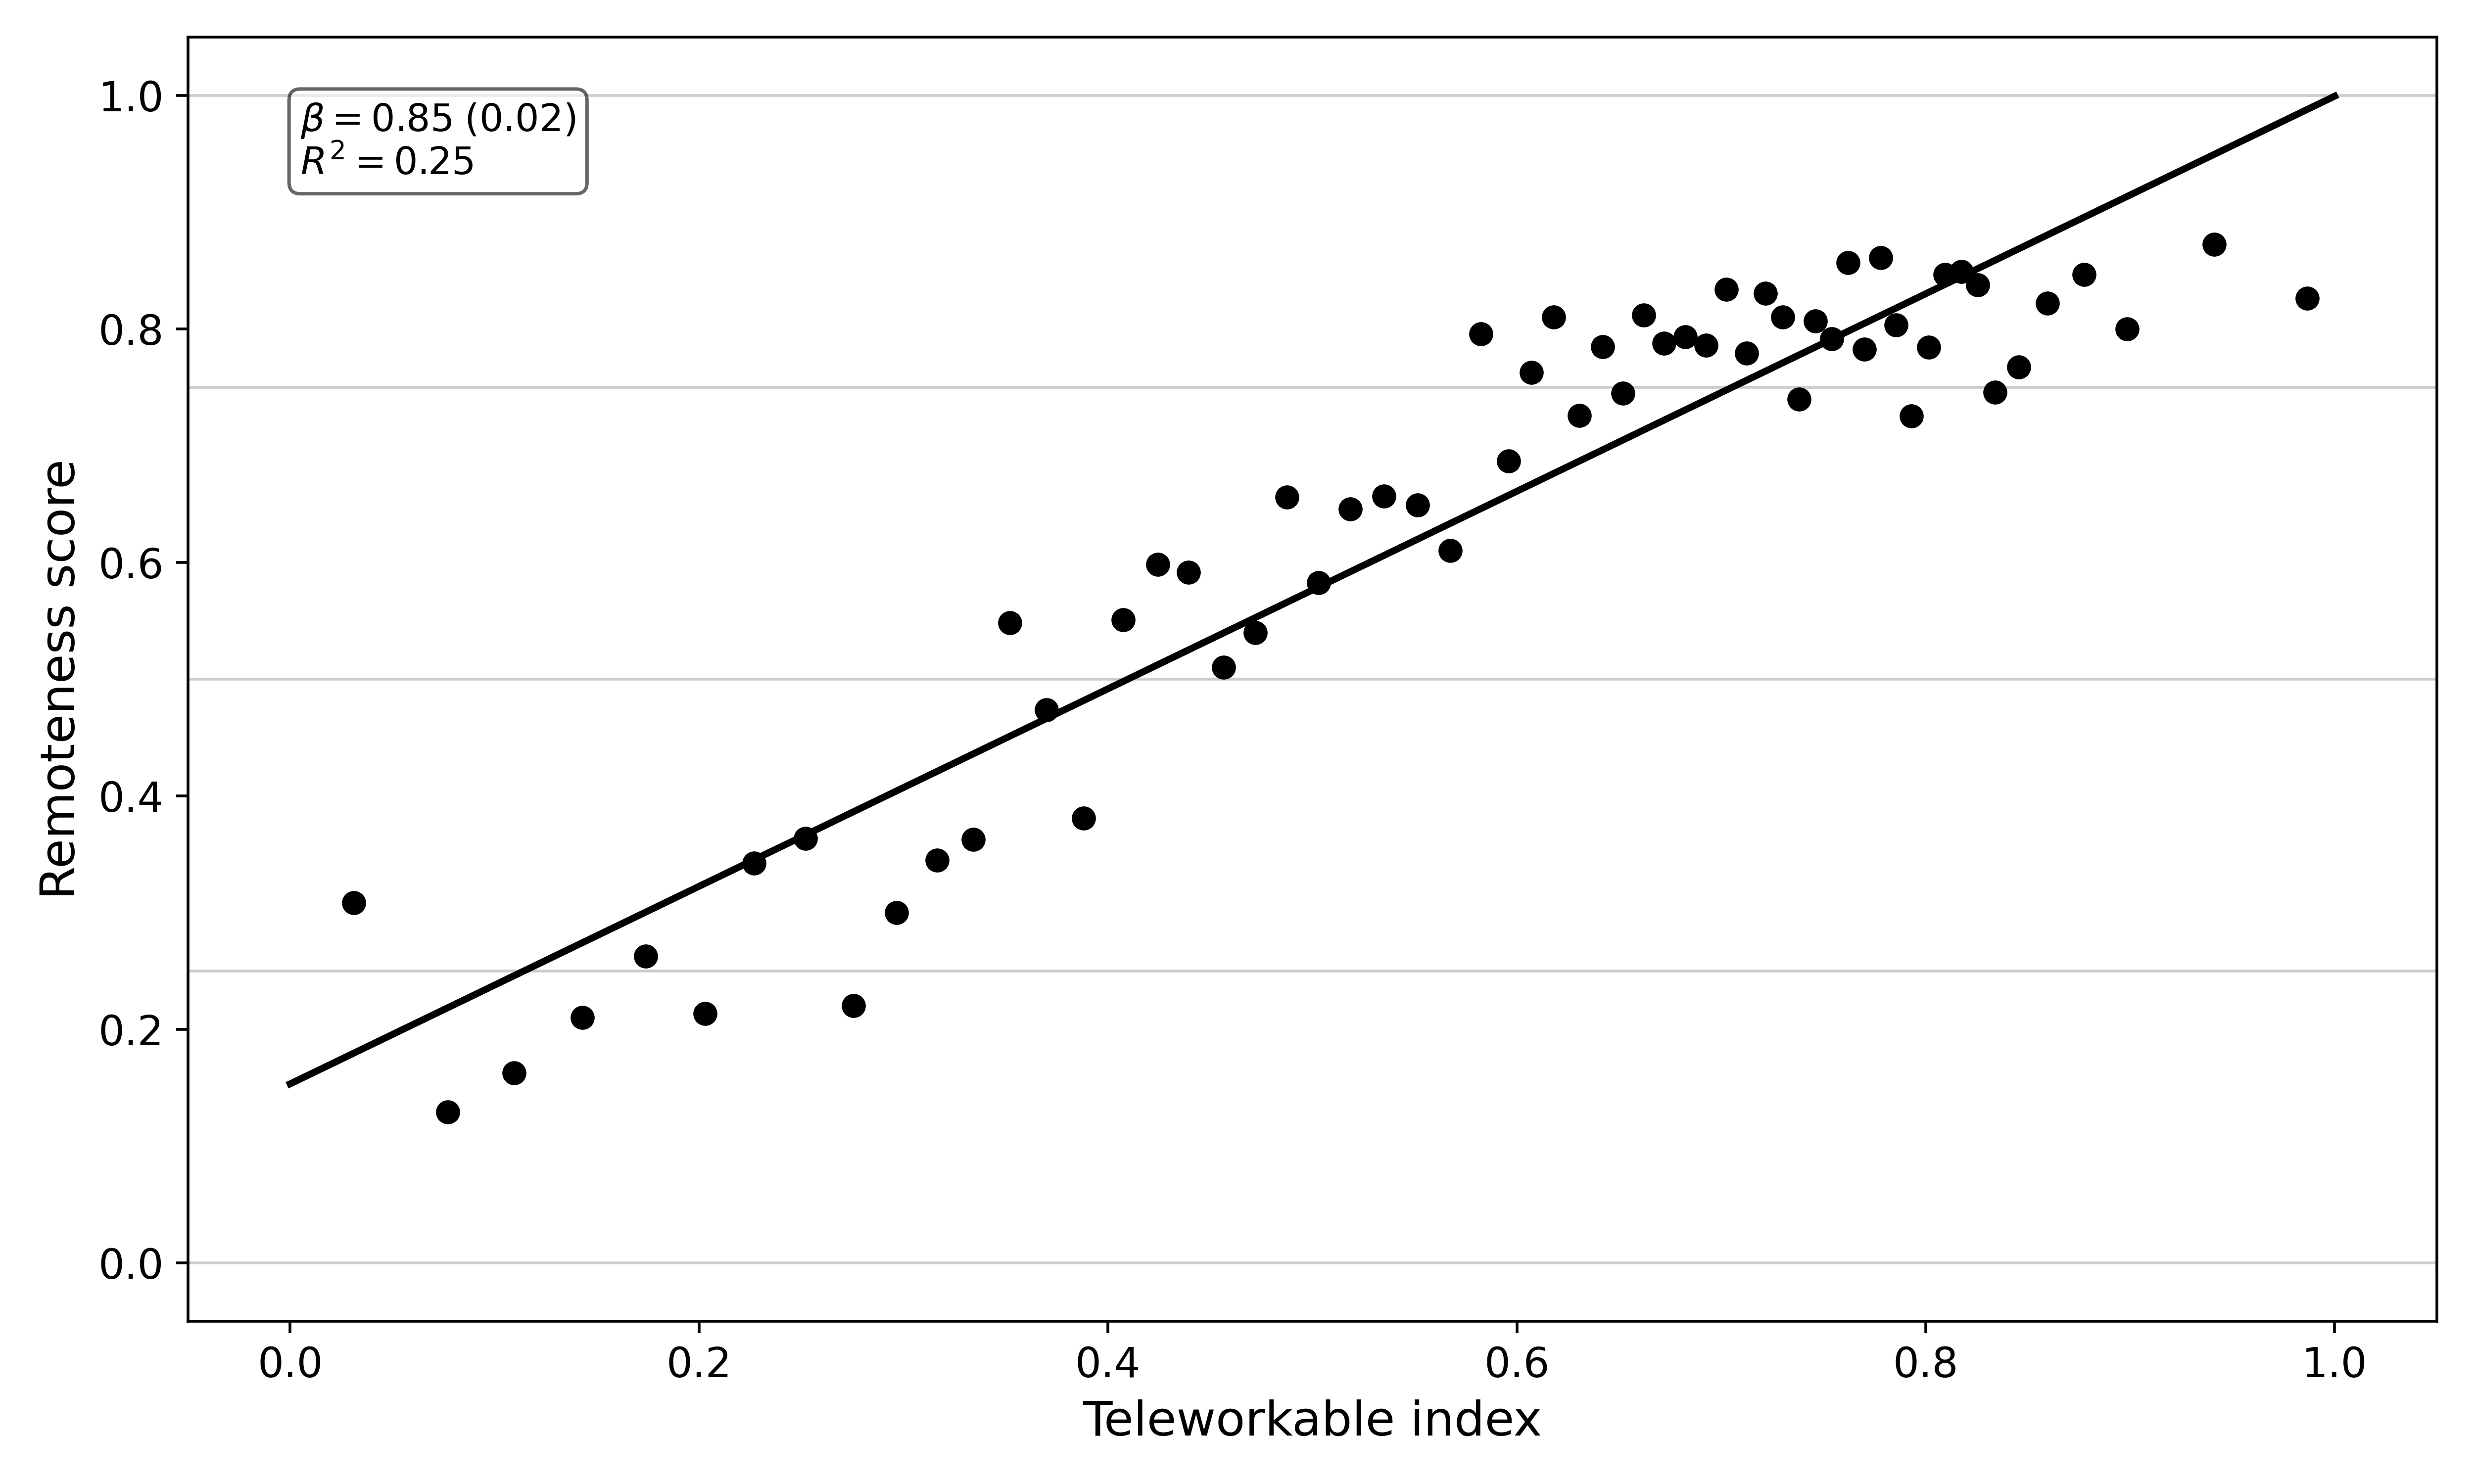
\includegraphics[scale=0.4]{\figdir/firm_teleworkable_remote.png}
  \caption{Remote v. Teleworkabe Scores}
\end{figure}

\begin{figure}[H]
  \centering
  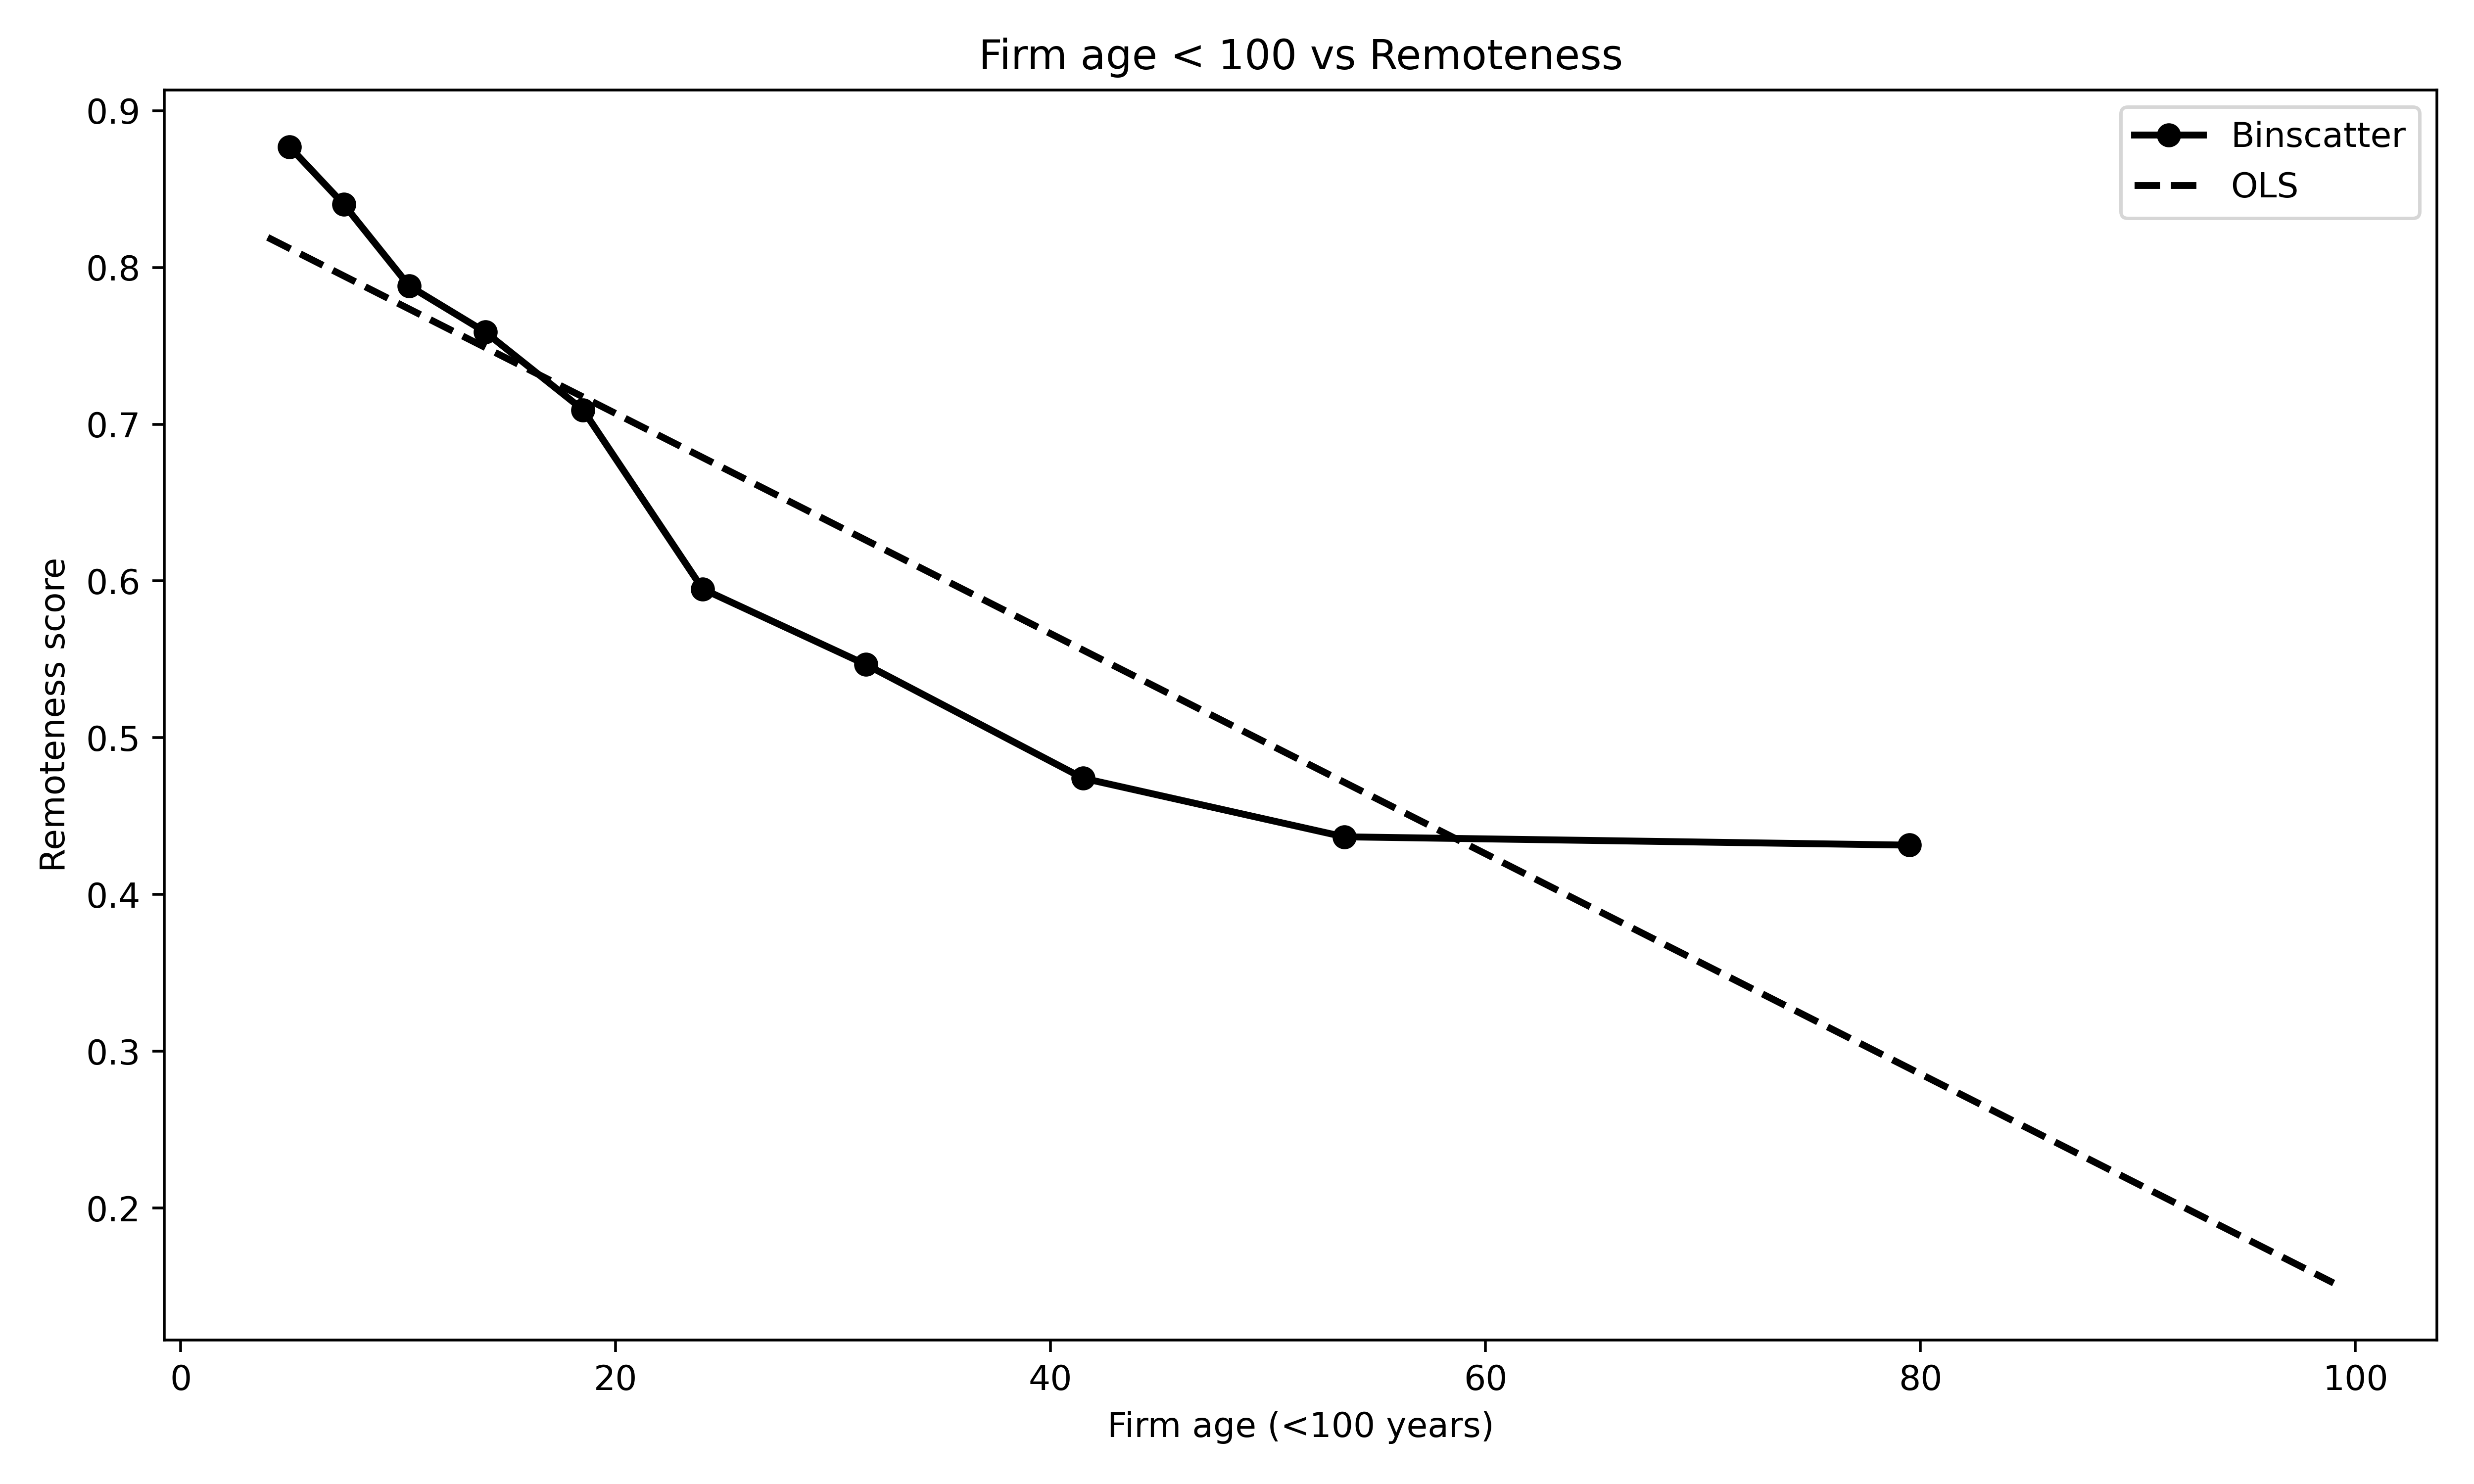
\includegraphics[scale=0.4]{\figdir/firm_age_lt100_remote.png}
  \caption{Remote v. Firm Age}
\end{figure}



\section{Table of Means}
\begin{table}[H]
        \centering
        \begin{threeparttable}
        \caption{Table of Means}
        \label{tab:means}
        \begin{tabular}{lcc@{\hspace{6pt}}c}
        \toprule
         & Startup & Incumbent & All Firms \\
        \midrule
        \addlinespace
        \multicolumn{4}{l}{\textbf{\uline{Panel A: Firm-level}}}\\[0.3em]
        Growth & \makecell{0.20 \\ (0.31)} & \makecell{0.06 \\ (0.16)} & \makecell{0.09 \\ (0.22)} \\
Leave & \makecell{0.26 \\ (0.31)} & \makecell{0.21 \\ (0.28)} & \makecell{0.22 \\ (0.29)} \\
Join & \makecell{0.35 \\ (0.32)} & \makecell{0.17 \\ (0.18)} & \makecell{0.22 \\ (0.24)} \\
Teleworkable Score \,(0--1) & \makecell{0.67 \\ (0.18)} & \makecell{0.54 \\ (0.25)} & \makecell{0.57 \\ (0.24)} \\
Remote Score \,(0--1) & \makecell{0.85 \\ (0.30)} & \makecell{0.57 \\ (0.41)} & \makecell{0.64 \\ (0.40)} \\
Employees (Count) & \makecell{271 \\ (1432)} & \makecell{2740 \\ (9555)} & \makecell{2126 \\ (8380)} \\
Age & \makecell{7 \\ (2)} & \makecell{43 \\ (34)} & \makecell{34 \\ (33)} \\
Rent (\textdollar/sq ft) & \makecell{49 \\ (21)} & \makecell{37 \\ (19)} & \makecell{40 \\ (20)} \\
Centrality Score & \makecell{1419 \\ (1830)} & \makecell{949 \\ (1309)} & \makecell{1066 \\ (1470)} \\
Seniority Levels (Count) & \makecell{3.62 \\ (0.77)} & \makecell{3.86 \\ (0.50)} & \makecell{3.80 \\ (0.59)} \\
\addlinespace
\midrule
Number of firms & 878 & 2630 & 3508 \\
Observations & 10450 & 31530 & 41980 \\
        \addlinespace
        \midrule
        \addlinespace
        \multicolumn{4}{l}{\textbf{\uline{Panel B: User-level}}}\\[0.3em]
        Total Contributions & \makecell{363.55 \\ (796.33)} & \makecell{193.43 \\ (641.42)} & \makecell{225.69 \\ (676.83)} \\
Restricted Contributions & \makecell{319.21 \\ (727.47)} & \makecell{138.68 \\ (356.21)} & \makecell{172.91 \\ (456.26)} \\
\addlinespace
\midrule
Number of firms & 727 & 1530 & 2257 \\
Number of users & 8635 & 33351 & 38411 \\
Observations & 48756 & 208390 & 257146 \\
        \bottomrule
        \end{tabular}
        \begin{tablenotes}[flushleft]
\footnotesize
\item \emph{Notes}: Panel~A uses firm--half--year observations. Panel~B relies on worker--half--year observations. ``Number of firms'' counts distinct firm\,IDs that ever appear in each category over the full sample window, so Startup and Incumbent counts need not sum to the ``All'' column. \textit{Growth}, \textit{Leave}, and \textit{Join} rates are fractions between 0 and 1. \textit{Teleworkable} and \textit{Remote} scores are index values between~0 and~1.  The sample period spans 2016 H2–2022 H1 at the firm level and 2017 H1–2022 H1 at the user level.
\end{tablenotes}
        \end{threeparttable}
        \end{table}
%
% -------------------------------------------------------------------------
%  User productivity – Pre-COVID (main headline results)
% -------------------------------------------------------------------------
\section{User Productivity – Pre-COVID Panel}

\subsection{OLS}
\begin{table}[H]
\centering
{\scriptsize\centering
  \caption{User Productivity -- OLS}
  \label{tab:user_productivity_precovid_ols}
}
\centering
{\scriptsize%
\setlength{\tabcolsep}{3pt}%
\renewcommand{\arraystretch}{0.95}%
\begin{adjustbox}{max width=\linewidth, max height=0.9\textheight, center}%

\begin{tabularx}{\linewidth}{l@{\hspace{4pt}}>{\centering\arraybackslash}X@{\hspace{4pt}}@{\hspace{4pt}}>{\centering\arraybackslash}X@{\hspace{4pt}}@{\hspace{4pt}}>{\centering\arraybackslash}X@{\hspace{4pt}}@{\hspace{4pt}}>{\centering\arraybackslash}X@{\hspace{4pt}}@{\hspace{4pt}}>{\centering\arraybackslash}X@{\hspace{4pt}}@{\hspace{4pt}}>{\centering\arraybackslash}X@{\hspace{4pt}}}
\toprule
 & (1) & (2) & (3) & (4) & (5) & (6) \\
\midrule
 & \makecell[c]{Total\\(pct.\ rk.)} & \makecell[c]{Total\\(pct.\ rk.)} & \makecell[c]{Total\\(pct.\ rk.)} & \makecell[c]{Restr.\\(pct.\ rk.)} & \makecell[c]{Total\\(wins.)} & \makecell[c]{Restr.\\(wins.)} \\
\midrule
$ \text{Remote} \times \mathds{1}(\text{Post}) $ & \makecell[c]{-0.28\\(0.44)} & \makecell[c]{-1.03**\\(0.48)} & \makecell[c]{-1.23**\\(0.50)} & \makecell[c]{-1.48***\\(0.52)} & \makecell[c]{-19.74***\\(4.66)} & \makecell[c]{-17.33***\\(3.91)} \\
$ \text{Remote} \times \mathds{1}(\text{Post}) \times \text{Startup} $ &  & \makecell[c]{5.18***\\(1.24)} & \makecell[c]{6.21***\\(1.27)} & \makecell[c]{7.31***\\(1.27)} & \makecell[c]{59.23***\\(14.22)} & \makecell[c]{55.41***\\(12.74)} \\
\midrule
Time FE & $\checkmark$ & $\checkmark$ & $\checkmark$ & $\checkmark$ & $\checkmark$ & $\checkmark$ \\
Firm FE & $\checkmark$ & $\checkmark$ &  &  &  &  \\
User FE & $\checkmark$ & $\checkmark$ &  &  &  &  \\
Firm $\times$ User FE &  &  & $\checkmark$ & $\checkmark$ & $\checkmark$ & $\checkmark$ \\
\midrule
    Pre-COVID mean & 49.92 & 49.92 & 49.92 & 48.48 & 184.71 & 138.15 \\

    N & 229,862 & 229,862 & 224,708 & 224,708 & 224,708 & 224,708 \\
\bottomrule
\end{tabularx}\end{adjustbox}}
\end{table}


\subsection{Instrumental Variables}
% Auto-generated user productivity table

\begin{table}[H]
\centering
\caption{User Productivity (precovid) -- IV}
\label{tab:user_productivity_precovid_iv}
\centering

    \begin{tabularx}{\dimexpr\textwidth + 2cm\relax}{@{}l@{\hskip 8pt}>{\centering\arraybackslash}X@{\hskip 8pt}>{\centering\arraybackslash}X@{\hskip 8pt}>{\centering\arraybackslash}X@{\hskip 8pt}>{\centering\arraybackslash}X@{\hskip 8pt}>{\centering\arraybackslash}X@{\hskip 8pt}>{\centering\arraybackslash}X@{}}
    \toprule
    \multicolumn{7}{@{}l}{\textbf{\uline{Panel A: Total Contrib. (pct. rk)}}}\\
\addlinespace


     & (1) & (2) & (3) & (4) & (5) & (6) \\
    \midrule
    $ \text{Remote} \times \mathds{1}(\text{Post}) $ & \makecell[c]{4.10\\(2.74)} & \makecell[c]{3.88\\(4.00)} & \makecell[c]{2.24\\(4.04)} & \makecell[c]{10.69**\\(5.44)} & \makecell[c]{3.83\\(4.30)} & \makecell[c]{8.99\\(8.33)} \\
$ \text{Remote} \times \mathds{1}(\text{Post}) \times \text{Startup} $ &  & \makecell[c]{0.61\\(4.86)} & \makecell[c]{1.16\\(4.78)} & \makecell[c]{-3.35\\(4.68)} & \makecell[c]{0.39\\(5.41)} & \makecell[c]{-4.77\\(6.46)} \\
    \midrule
    Time FE & $\checkmark$ & $\checkmark$ & $\checkmark$ &  &  &  \\
Firm FE & $\checkmark$ & $\checkmark$ &  & $\checkmark$ & $\checkmark$ & $\checkmark$ \\
User FE & $\checkmark$ & $\checkmark$ &  & $\checkmark$ & $\checkmark$ & $\checkmark$ \\
Firm $\times$ User FE &  &  & $\checkmark$ &  &  &  \\
Industry $\times$ Time FE &  &  &  & $\checkmark$ &  & $\checkmark$ \\
MSA $\times$ Time FE &  &  &  &  & $\checkmark$ & $\checkmark$ \\
    \midrule
    N & 229,862 & 229,862 & 224,708 & 227,829 & 229,043 & 222,867 \\
KP rk Wald F & 543.26 & 140.60 & 123.43 & 109.16 & 130.48 & 49.49 \\
    \specialrule{\lightrulewidth}{0pt}{0pt}
    \end{tabularx}

    \begin{tabularx}{\dimexpr\textwidth + 2cm\relax}{@{}l@{\hskip 8pt}>{\centering\arraybackslash}X@{\hskip 8pt}>{\centering\arraybackslash}X@{\hskip 8pt}>{\centering\arraybackslash}X@{}}

    \multicolumn{4}{@{}l}{\textbf{\uline{Panel B: Additional Outcomes}}}\\
\addlinespace
     & \multicolumn{3}{c}{Outcome} \\
    \cmidrule(lr){2-4}
     & Restricted (pct. rk) & Total (wins.) & Restr. (wins.) \\
    \midrule
    $ \text{Remote} \times \mathds{1}(\text{Post}) $ & \makecell[c]{5.65\\(4.80)} & \makecell[c]{-51.50***\\(17.23)} & \makecell[c]{-43.05***\\(11.69)} \\
$ \text{Remote} \times \mathds{1}(\text{Post}) \times \text{Startup} $ & \makecell[c]{-2.61\\(5.67)} & \makecell[c]{62.77**\\(26.20)} & \makecell[c]{53.17***\\(17.41)} \\
    \midrule
    Pre-COVID mean & 75.54 & 126.64 & 77.02 \\
    N & 229,862 & 229,862 & 229,862 \\
    KP rk Wald F & 140.60 & 140.60 & 140.60 \\
    \bottomrule
    \end{tabularx}
\end{table}


\subsection{First Stage}
% Auto-generated – do *not* edit by hand
\begin{table}[H]
\centering
\caption{First-Stage Estimates -- User Productivity (precovid)}
\label{tab:user_productivity_precovid_first_stage}
\begin{tabular}{lcc}
\toprule
 & $ \text{Remote} \times \mathds{1}(\text{Post}) $ & $ \text{Remote} \times \mathds{1}(\text{Post}) \times \text{Startup} $\\
\midrule
$ \text{Teleworkable} \times \mathds{1}(\text{Post}) $ & \makecell[c]{0.23***\\(0.01)} & \makecell[c]{-0.00*\\(0.00)}\\
$ \text{Teleworkable} \times \mathds{1}(\text{Post}) \times \text{Startup} $ & \makecell[c]{0.16***\\(0.02)} & \makecell[c]{0.39***\\(0.02)}\\
$ \mathds{1}(\text{Post}) \times \text{Startup} $ & \makecell[c]{0.09***\\(0.02)} & \makecell[c]{0.60***\\(0.01)}\\
\midrule
Time FE & $\checkmark$ & $\checkmark$\\
Firm FE & $\checkmark$ & $\checkmark$\\
User FE & $\checkmark$ & $\checkmark$\\
\midrule
Partial F & 323.23 & 187.25\\
N & 245,105 & 245,105\\
\bottomrule
\end{tabular}
\end{table}



% \subsection{Weighted Sample}
% % Auto-generated table from consolidated_results.csv
\begin{table}[H]
\caption{User Productivity Precovid Weighted}
\label{tab:user_productivity_precovid_weighted}
\centering
\begin{tabular}{lll}
\toprule
Parameter & IV & OLS \\
\midrule
$ \text{Remote} \times \mathds{1}(\text{Post}) $ & \makecell[c]{-6.878\\(9.803)} & \makecell[c]{0.014\\(1.037)} \\
$ \text{Remote} \times \mathds{1}(\text{Post}) \times \text{Startup} $ & \makecell[c]{15.819\\(10.829)} & \makecell[c]{8.950***\\(2.643)} \\
$ \mathds{1}(\text{Post}) \times \text{Startup} $ & \makecell[c]{-10.954*\\(6.596)} & \makecell[c]{-7.004***\\(2.033)} \\
\bottomrule
\end{tabular}
\end{table}


% Additional pre-COVID variants (commented out)
% \subsection{Full Remote Variant}
% % Auto-generated table from consolidated_results.csv
\begin{table}[H]
\caption{User Productivity Precovid Fullremote}
\label{tab:user_productivity_precovid_fullremote}
\centering
\begin{tabular}{lll}
\toprule
Parameter & IV & OLS \\
\midrule
$ \text{Remote} \times \mathds{1}(\text{Post}) $ & \makecell[c]{-3.089*\\(1.675)} & \makecell[c]{-0.675**\\(0.300)} \\
$ \text{Remote} \times \mathds{1}(\text{Post}) \times \text{Startup} $ & \makecell[c]{4.385*\\(2.409)} & \makecell[c]{2.806***\\(0.692)} \\
$ \mathds{1}(\text{Post}) \times \text{Startup} $ & \makecell[c]{-3.293**\\(1.370)} & \makecell[c]{-3.045***\\(0.548)} \\
\bottomrule
\end{tabular}
\end{table}


% \subsection{Hybrid Variant}
% % Auto-generated table from consolidated_results.csv
\begin{table}[H]
\caption{User Productivity Precovid Hybrid}
\label{tab:user_productivity_precovid_hybrid}
\centering
\begin{tabular}{lll}
\toprule
Parameter & IV & OLS \\
\midrule
$ \text{Remote} \times \mathds{1}(\text{Post}) $ & \makecell[c]{3.540*\\(1.919)} & \makecell[c]{0.834***\\(0.291)} \\
$ \text{Remote} \times \mathds{1}(\text{Post}) \times \text{Startup} $ & \makecell[c]{-5.011*\\(2.755)} & \makecell[c]{-2.186***\\(0.700)} \\
$ \mathds{1}(\text{Post}) \times \text{Startup} $ & \makecell[c]{1.159\\(1.297)} & \makecell[c]{-0.470\\(0.406)} \\
\bottomrule
\end{tabular}
\end{table}


% -------------------------------------------------------------------------
%  Lean mechanism horse-race (Pre-COVID only)
% -------------------------------------------------------------------------
\clearpage
\begin{landscape}
\section{User Mechanisms – Covid Bifurcation (Continuous) – Pre-COVID Panel}
\begin{table}[H]
\centering
\caption{User Mechanisms – Lean (Precovid) – Part 1}
\begin{tabular}{lcccccc}
\toprule
 & \multicolumn{6}{c}{Total Contrib. (pct. rk)} \\
\cmidrule(lr){2-7}
Specification & (1) & (2) & (3) & (4) & (5) & (6) \\
\midrule
Rent &  & \checkmark &  &  & \checkmark & \checkmark \\
HHI &  &  & \checkmark &  & \checkmark &  \\
Seniority &  &  &  & \checkmark &  & \checkmark \\
\midrule
\multicolumn{7}{l}{\textbf{\uline{Panel A: OLS}}} \\
\addlinespace
$ \text{Remote} \times \mathds{1}(\text{Post}) $ & -1.23** & -0.95* & -1.22** & -1.08** & -0.95* & -0.90* \\
 & (0.50) & (0.51) & (0.50) & (0.51) & (0.51) & (0.52) \\
$ \text{Remote} \times \mathds{1}(\text{Post}) \times \text{Startup} $ & 6.21*** & 4.03*** & 6.39*** & 6.76*** & 4.21*** & 4.62*** \\
 & (1.27) & (1.26) & (1.28) & (1.32) & (1.27) & (1.31) \\
\midrule
N & 224,708 & 218,112 & 224,596 & 224,708 & 218,032 & 218,112 \\
\midrule
\multicolumn{7}{l}{\textbf{\uline{Panel B: IV}}} \\
\addlinespace
$ \text{Remote} \times \mathds{1}(\text{Post}) $ & -9.26** & -9.23* & -9.72** & -13.82* & -9.97** & -15.05* \\
 & (4.01) & (4.87) & (3.93) & (7.80) & (4.86) & (8.88) \\
$ \text{Remote} \times \mathds{1}(\text{Post}) \times \text{Startup} $ & 12.45** & 11.76* & 14.94*** & 26.14*** & 14.35** & 26.68** \\
 & (5.39) & (6.15) & (5.62) & (10.10) & (6.49) & (11.32) \\
\midrule
N & 224,708 & 218,112 & 224,596 & 224,708 & 218,032 & 218,112 \\
KP\,rk Wald F & 123.43 & 81.62 & 130.14 & 30.71 & 82.68 & 24.19 \\
\bottomrule
\end{tabular}
\label{tab:user_mechanisms_lean_precovid_1}
\end{table}

\end{landscape}

% -------------------------------------------------------------------------
%  Lean Binned user mechanisms
% -------------------------------------------------------------------------
\clearpage
\begin{landscape}
\section{User Mechanisms – Covid Bifurcation (Binned) – Pre-COVID Panel}
\begin{table}[H]
\centering
\caption{User Mechanisms – Lean (Precovid) – Part 1}
\begin{tabular}{lcccccccc}
\toprule
 & \multicolumn{8}{c}{Total Contrib. (pct. rk)} \\
\cmidrule(lr){2-9}
Specification & (1) & (2) & (3) & (4) & (5) & (6) & (7) & (8) \\
\midrule
Rent &  & \checkmark &  &  & \checkmark & \checkmark &  & \checkmark \\
HHI &  &  & \checkmark &  & \checkmark &  & \checkmark & \checkmark \\
Seniority &  &  &  & \checkmark &  & \checkmark & \checkmark & \checkmark \\
\midrule
\multicolumn{9}{l}{\textbf{\uline{Panel A: OLS}}} \\
\addlinespace
$ \text{Remote} \times \mathds{1}(\text{Post}) $ & -1.23** & -1.11* & -1.54** & 2.65 & -1.21* & 4.16 & 2.14 & 3.96 \\
 & (0.50) & (0.63) & (0.63) & (5.85) & (0.71) & (5.80) & (5.90) & (5.86) \\
$ \text{Remote} \times \mathds{1}(\text{Post}) \times \text{Startup} $ & 6.21*** & 4.08*** & 6.07*** & 6.09*** & 4.06*** & 3.90*** & 5.95*** & 3.88*** \\
 & (1.27) & (1.27) & (1.29) & (1.28) & (1.28) & (1.27) & (1.29) & (1.28) \\
\midrule
N & 224,708 & 218,112 & 224,596 & 224,708 & 218,032 & 218,112 & 224,596 & 218,032 \\
\midrule
\multicolumn{9}{l}{\textbf{\uline{Panel B: IV}}} \\
\addlinespace
$ \text{Remote} \times \mathds{1}(\text{Post}) $ & -9.26** & -990.04 & -188.00** & -21799.94 & -677.88 & 7540.44 & 5749.41 & 19936.89 \\
 & (4.01) & (3169.06) & (95.53) & (13665.66) & (982.93) & (13396.79) & (11264.50) & (149586.97) \\
$ \text{Remote} \times \mathds{1}(\text{Post}) \times \text{Startup} $ & 12.45** & -182.31 & -14.51 & -310.11 & 80.55 & 177.08 & 122.50 & -67.96 \\
 & (5.39) & (642.58) & (16.54) & (255.37) & (85.79) & (266.43) & (200.54) & (1452.16) \\
\midrule
N & 224,708 & 203,754 & 209,684 & 209,788 & 203,676 & 203,754 & 209,684 & 203,676 \\
KP\,rk Wald F & 123.43 & 0.03 & 2.18 & 0.96 & 0.17 & 0.09 & 0.07 & 0.00 \\
\bottomrule
\end{tabular}
\label{tab:user_mechanisms_lean_precovid_1}
\end{table}

\end{landscape}

% -------------------------------------------------------------------------
%  Full horse‐race mechanisms (Pre-COVID) – include both OLS & IV panels
% -------------------------------------------------------------------------
\clearpage
\begin{landscape}
\section{User Mechanisms – Remote Bifurcation (Continuous) – Pre-COVID Panel}
\begin{table}[H]
\centering
\caption{User Mechanisms (Precovid) – Part 1}
\begin{tabular}{lcccccccc}
\toprule
 & \multicolumn{8}{c}{Total Contrib. (pct. rk)} \\
\cmidrule(lr){2-9}
Specification & (1) & (2) & (3) & (4) & (5) & (6) & (7) & (8) \\
\midrule
Rent &  & \checkmark &  &  & \checkmark & \checkmark &  & \checkmark \\
HHI &  &  & \checkmark &  & \checkmark &  & \checkmark & \checkmark \\
Seniority &  &  &  & \checkmark &  & \checkmark & \checkmark & \checkmark \\
\midrule
\multicolumn{9}{l}{\textbf{\uline{Panel A: OLS}}} \\
\addlinespace
$ \text{Remote} \times \mathds{1}(\text{Post}) $ & -1.03** & -1.94* & -0.57 & 4.11 & -1.48 & 4.59 & 5.55 & 6.04 \\
 & (0.48) & (1.13) & (0.60) & (5.86) & (1.18) & (5.86) & (5.95) & (5.94) \\
$ \text{Remote} \times \mathds{1}(\text{Post}) \times \text{Startup} $ & 5.25*** & 2.91** & 5.64*** & 5.10*** & 3.35*** & 2.71** & 5.47*** & 3.12** \\
 & (1.24) & (1.24) & (1.29) & (1.24) & (1.28) & (1.24) & (1.29) & (1.28) \\
\midrule
N & 229,710 & 222,851 & 229,620 & 229,710 & 222,798 & 222,851 & 229,620 & 222,798 \\
\midrule
\multicolumn{9}{l}{\textbf{\uline{Panel B: IV}}} \\
\addlinespace
$ \text{Remote} \times \mathds{1}(\text{Post}) $ & -4.57 & -2775.24 & -98.17 & 88633.78 & 2183.05 & 39.59 & 5246.00 & 1651.21 \\
 & (3.39) & (11069.18) & (198.56) & (356887.66) & (9557.95) & (4560.50) & (17096.43) & (1963.50) \\
$ \text{Remote} \times \mathds{1}(\text{Post}) \times \text{Startup} $ & 9.78* & 259.56 & -27.25 & 2571.92 & -254.15 & 196.96 & 239.35 & 18.19 \\
 & (5.44) & (1034.96) & (77.53) & (10384.31) & (1451.85) & (446.61) & (527.34) & (505.58) \\
\midrule
N & 229,710 & 208,057 & 214,249 & 214,330 & 208,006 & 208,057 & 214,249 & 208,006 \\
KP\,rk Wald F & 180.13 & 0.02 & 0.08 & 0.02 & 0.01 & 0.04 & 0.04 & 0.02 \\
\bottomrule
\end{tabular}
\label{tab:user_mechanisms_precovid_1}
\end{table}

\end{landscape}

% -------------------------------------------------------------------------
%  Binned horse‐race mechanisms (Pre-COVID) – NEW
% -------------------------------------------------------------------------
\clearpage
\begin{landscape}
\section{User Mechanisms – Remote Bifurcation (Binned) – Pre-COVID Panel}
\begin{table}[H]
\centering
\caption{User Mechanisms (Precovid) – Part 1}
\begin{tabular}{lcccccccc}
\toprule
 & \multicolumn{8}{c}{Total Contrib. (pct. rk)} \\
\cmidrule(lr){2-9}
Specification & (1) & (2) & (3) & (4) & (5) & (6) & (7) & (8) \\
\midrule
Rent &  & \checkmark &  &  & \checkmark & \checkmark &  & \checkmark \\
HHI &  &  & \checkmark &  & \checkmark &  & \checkmark & \checkmark \\
Seniority &  &  &  & \checkmark &  & \checkmark & \checkmark & \checkmark \\
\midrule
\multicolumn{9}{l}{\textbf{\uline{Panel A: OLS}}} \\
\addlinespace
$ \text{Remote} \times \mathds{1}(\text{Post}) $ & -1.23** & -1.11* & -1.54** & 2.65 & -1.21* & 4.16 & 2.14 & 3.96 \\
 & (0.50) & (0.63) & (0.63) & (5.85) & (0.71) & (5.80) & (5.90) & (5.86) \\
$ \text{Remote} \times \mathds{1}(\text{Post}) \times \text{Startup} $ & 6.21*** & 4.08*** & 6.07*** & 6.09*** & 4.06*** & 3.90*** & 5.95*** & 3.88*** \\
 & (1.27) & (1.27) & (1.29) & (1.28) & (1.28) & (1.27) & (1.29) & (1.28) \\
\midrule
N & 224,708 & 218,112 & 224,596 & 224,708 & 218,032 & 218,112 & 224,596 & 218,032 \\
\midrule
\multicolumn{9}{l}{\textbf{\uline{Panel B: IV}}} \\
\addlinespace
$ \text{Remote} \times \mathds{1}(\text{Post}) $ & -9.26** & -990.04 & -188.00** & -21799.94 & -677.88 & 7540.44 & 5749.41 & 19936.89 \\
 & (4.01) & (3169.06) & (95.53) & (13665.66) & (982.93) & (13396.79) & (11264.50) & (149586.97) \\
$ \text{Remote} \times \mathds{1}(\text{Post}) \times \text{Startup} $ & 12.45** & -182.31 & -14.51 & -310.11 & 80.55 & 177.08 & 122.50 & -67.96 \\
 & (5.39) & (642.58) & (16.54) & (255.37) & (85.79) & (266.43) & (200.54) & (1452.16) \\
\midrule
N & 224,708 & 203,754 & 209,684 & 209,788 & 203,676 & 203,754 & 209,684 & 203,676 \\
KP\,rk Wald F & 123.43 & 0.03 & 2.18 & 0.96 & 0.17 & 0.09 & 0.07 & 0.00 \\
\bottomrule
\end{tabular}
\label{tab:user_mechanisms_precovid_1}
\end{table}

\end{landscape}

% -------------------------------------------------------------------------
%  Firm results (mirroring the consolidated report)
% -------------------------------------------------------------------------

\clearpage
\section{Firm Scaling}

\subsection{OLS}
% ------------------------------------------------------------------
%  Firm-Scaling: Two-panel OLS results
% ------------------------------------------------------------------

\begin{table}[H]
\centering
\caption{Firm Scaling OLS}
\label{tab:firm_scaling_ols}
\centering

    \begin{tabular*}{\textwidth}{@{}l@{\extracolsep{\fill}}cccc@{}}
    \toprule
    \multicolumn{5}{@{}l}{\textbf{\uline{Panel A: FE Variants}}}\\
\addlinespace
     & \multicolumn{4}{c}{Growth} \\
    \cmidrule(lr){2-5}
     & (1) & (2) & (3) & (4) \\
    \midrule
    $ \text{Remote} \times \mathds{1}(\text{Post}) $ & \makecell[c]{0.00\\(0.00)} & \makecell[c]{0.00\\(0.00)} & \makecell[c]{0.00\\(0.00)} & \makecell[c]{0.00\\(0.00)} \\
$ \text{Remote} \times \mathds{1}(\text{Post}) \times \text{Startup} $ & \makecell[c]{0.07***\\(0.02)} & \makecell[c]{0.07***\\(0.02)} & \makecell[c]{0.07***\\(0.02)} & \makecell[c]{0.07***\\(0.02)} \\
    \midrule
    Time FE &  &  & $\checkmark$ & $\checkmark$ \\
Firm FE &  & $\checkmark$ &  & $\checkmark$ \\
    \midrule
    N & 41,980 & 41,980 & 41,980 & 41,980 \\
    \specialrule{\lightrulewidth}{0pt}{0pt}
    \end{tabular*}
\vspace{0.75em}
\begin{tabular*}{\textwidth}{@{}l@{\extracolsep{\fill}}ccc@{}}

    \multicolumn{4}{@{}l}{\textbf{\uline{Panel B: Base Specification}}}\\
\addlinespace
     & \multicolumn{3}{c}{Outcome} \\
    \cmidrule(lr){2-4}
     & Growth & Join & Leave \\
    \midrule
    $ \text{Remote} \times \mathds{1}(\text{Post}) $ & \makecell[c]{0.00\\(0.00)} & \makecell[c]{0.01**\\(0.00)} & \makecell[c]{0.02***\\(0.00)} \\
$ \text{Remote} \times \mathds{1}(\text{Post}) \times \text{Startup} $ & \makecell[c]{0.07***\\(0.02)} & \makecell[c]{0.05*\\(0.03)} & \makecell[c]{-0.01\\(0.01)} \\
    \midrule
    N & 41,980 & 41,980 & 41,980 \\
    \bottomrule
    \end{tabular*}
\end{table}


\subsection{Instrumental Variables}
\begin{table}[H]
\centering
{\scriptsize\centering
  \caption{Firm Scaling — IV}
  \label{tab:firm_scaling_iv}
}
\centering
{\scriptsize%
\setlength{\tabcolsep}{3pt}%
\renewcommand{\arraystretch}{0.95}%
\begin{adjustbox}{max width=\linewidth, max height=0.9\textheight, center}%

    \begin{tabularx}{\linewidth}{l@{\hspace{4pt}}>{\centering\arraybackslash}X@{\hspace{4pt}}@{\hspace{4pt}}>{\centering\arraybackslash}X@{\hspace{4pt}}@{\hspace{4pt}}>{\centering\arraybackslash}X@{\hspace{4pt}}@{\hspace{4pt}}>{\centering\arraybackslash}X@{\hspace{4pt}}}
    \toprule
     & (1) & (2) & (3) & (4) \\
    \midrule
     & \makecell[c]{Growth\\(wins.)} & \makecell[c]{Growth\\(wins.)} & \makecell[c]{Join\\(wins.)} & \makecell[c]{Leave\\(wins.)} \\
    \midrule
    $ \text{Remote} \times \mathds{1}(\text{Post}) $ & \makecell[c]{0.02\\(0.01)} & \makecell[c]{-0.00\\(0.01)} & \makecell[c]{0.03***\\(0.01)} & \makecell[c]{0.04***\\(0.00)} \\
$ \text{Remote} \times \mathds{1}(\text{Post}) \times \text{Startup} $ &  & \makecell[c]{0.22**\\(0.09)} & \makecell[c]{0.23**\\(0.10)} & \makecell[c]{0.06\\(0.05)} \\
    \midrule
    Time FE & $\checkmark$ & $\checkmark$ & $\checkmark$ & $\checkmark$ \\
Firm FE & $\checkmark$ & $\checkmark$ & $\checkmark$ & $\checkmark$ \\
    \midrule
    Pre-COVID mean & 0.11 & 0.11 & 0.25 & 0.14 \\
    N & 41,742 & 41,742 & 41,742 & 41,742 \\
    KP rk Wald F & 982.73 & 18.30 & 18.30 & 18.30 \\
    \bottomrule
    \end{tabularx}\end{adjustbox}}
\end{table}


\subsection{First Stage}
% Auto-generated first-stage estimates – Firm Scaling
\begin{table}[H]
\centering
\caption{First-Stage Estimates – Firm Scaling}
\label{tab:firm_scaling_first_stage}
\begin{tabular}{lcc}
\toprule
 & $ \text{Remote} \times \mathds{1}(\text{Post}) $ & $ \text{Remote} \times \mathds{1}(\text{Post}) \times \text{Startup} $\\
\midrule
$ \text{Teleworkable} \times \mathds{1}(\text{Post}) $ & \makecell[c]{0.826***\\(0.028)} & \makecell[c]{-0.000\\(0.000)}\\
$ \text{Teleworkable} \times \mathds{1}(\text{Post}) \times \text{Startup} $ & \makecell[c]{-0.412***\\(0.077)} & \makecell[c]{0.414***\\(0.072)}\\
$ \mathds{1}(\text{Post}) \times \text{Startup} $ & \makecell[c]{0.455***\\(0.055)} & \makecell[c]{0.575***\\(0.052)}\\
\midrule
Time FE & $\checkmark$ & $\checkmark$\\
Firm FE & $\checkmark$ & $\checkmark$\\
\midrule
Partial F & 437.86 & 16.54\\
N & 41,980 & 41,980\\
\bottomrule
\end{tabular}
\end{table}


% Additional firm-scaling variants omitted from mini report
% \subsection{Hybrid Variant}
% % Auto-generated table from consolidated_results.csv
\begin{table}[H]
\caption{Firm Scaling Hybrid}
\label{tab:firm_scaling_hybrid}
\centering
\begin{tabular}{lll}
\toprule
Parameter & IV & OLS \\
\midrule
$ \text{Remote} \times \mathds{1}(\text{Post}) $ & \makecell[c]{0.021\\(0.033)} & \makecell[c]{0.013***\\(0.004)} \\
$ \text{Remote} \times \mathds{1}(\text{Post}) \times \text{Startup} $ & \makecell[c]{-1.473\\(1.873)} & \makecell[c]{-0.046**\\(0.019)} \\
$ \mathds{1}(\text{Post}) \times \text{Startup} $ & \makecell[c]{0.198\\(0.320)} & \makecell[c]{-0.047***\\(0.008)} \\
\bottomrule
\end{tabular}
\end{table}


% \subsection{Full Remote Variant}
% % Auto-generated table from consolidated_results.csv
\begin{table}[H]
\caption{Firm Scaling Fullremote}
\label{tab:firm_scaling_fullremote}
\centering
\begin{tabular}{lll}
\toprule
Parameter & IV & OLS \\
\midrule
$ \text{Remote} \times \mathds{1}(\text{Post}) $ & \makecell[c]{0.007\\(0.011)} & \makecell[c]{-0.004\\(0.004)} \\
$ \text{Remote} \times \mathds{1}(\text{Post}) \times \text{Startup} $ & \makecell[c]{0.182**\\(0.091)} & \makecell[c]{0.055***\\(0.017)} \\
$ \mathds{1}(\text{Post}) \times \text{Startup} $ & \makecell[c]{-0.199***\\(0.069)} & \makecell[c]{-0.097***\\(0.015)} \\
\bottomrule
\end{tabular}
\end{table}


% Remote vs. Teleworkable first stage
\subsection{Remote $\rightarrow$ Teleworkable: First Stage}
% Auto-generated – Remote on Teleworkable first stage
\begin{table}[H]
\centering
\caption{First-Stage Estimate: Remote $\rightarrow$ Teleworkable}
\label{tab:remote_first_stage}
\begin{tabular}{lc}
\toprule
 & $ \text{Remote} $\\
\midrule
$ \text{Teleworkable} $ & \makecell[c]{0.795***\\(0.021)}\\
\midrule
$R^2$ & 0.290\\
N & 3,486\\
\bottomrule
\end{tabular}
\end{table}


% Firm mechanisms ----------------------------------------------------------
% Firm mechanisms ----------------------------------------------------------
\clearpage
% Covid-Bifurcation (Lean) – Continuous
\begin{landscape}
\subsection{Firm Mechanisms – Covid Bifurcation (Continuous)}
\begin{table}[H]
\centering
\caption{Firm Mechanisms – Lean (Part 1)}
\begin{tabular}{lcccccccc}
\toprule
 & \multicolumn{8}{c}{Growth Rate} \\
\cmidrule(lr){2-9}
Specification & (1) & (2) & (3) & (4) & (5) & (6) & (7) & (8) \\
\midrule
Rent &  & \checkmark &  &  & \checkmark & \checkmark &  & \checkmark \\
HHI &  &  & \checkmark &  & \checkmark &  & \checkmark & \checkmark \\
Seniority &  &  &  & \checkmark &  & \checkmark & \checkmark & \checkmark \\
\midrule
\multicolumn{9}{l}{\textbf{\uline{Panel A: OLS}}} \\
\addlinespace
$ \text{Remote} \times \mathds{1}(\text{Post}) $ & 0.003 & 0.003 & 0.004 & 0.001 & 0.004 & 0.001 & 0.000 & 0.000 \\
 & (0.005) & (0.005) & (0.005) & (0.005) & (0.005) & (0.005) & (0.005) & (0.005) \\
$ \text{Remote} \times \mathds{1}(\text{Post}) \times \text{Startup} $ & 0.070*** & 0.067*** & 0.066*** & 0.070*** & 0.061** & 0.066*** & 0.070*** & 0.065*** \\
 & (0.024) & (0.025) & (0.024) & (0.023) & (0.025) & (0.025) & (0.023) & (0.025) \\
\midrule
N & 41,980 & 38,794 & 41,946 & 41,980 & 38,760 & 38,794 & 41,946 & 38,760 \\
\midrule
\multicolumn{9}{l}{\textbf{\uline{Panel B: IV}}} \\
\addlinespace
$ \text{Remote} \times \mathds{1}(\text{Post}) $ & 0.006 & 0.013 & 0.008 & 0.003 & 0.015 & 0.009 & 0.002 & 0.008 \\
 & (0.009) & (0.010) & (0.010) & (0.009) & (0.010) & (0.010) & (0.010) & (0.010) \\
$ \text{Remote} \times \mathds{1}(\text{Post}) \times \text{Startup} $ & 0.209** & 0.207* & 0.188* & 0.121 & 0.182 & 0.105 & 0.130 & 0.113 \\
 & (0.102) & (0.113) & (0.102) & (0.094) & (0.115) & (0.105) & (0.095) & (0.107) \\
\midrule
N & 41,980 & 38,794 & 41,946 & 41,980 & 38,760 & 38,794 & 41,946 & 38,760 \\
KP\,rk Wald F & 16.53 & 14.39 & 15.27 & 16.46 & 13.05 & 14.37 & 15.67 & 13.57 \\
\bottomrule
\end{tabular}
\label{tab:firm_mechanisms_lean_1}
\end{table}

\end{landscape}

% Covid-Bifurcation (Lean) – Binned
\begin{landscape}
\subsection{Firm Mechanisms – Covid Bifurcation (Binned)}
\begin{table}[H]
\centering
\caption{Firm Mechanisms – Lean (Part 1)}
\begin{tabular}{lcccccccc}
\toprule
 & \multicolumn{8}{c}{Growth Rate} \\
\cmidrule(lr){2-9}
Specification & (1) & (2) & (3) & (4) & (5) & (6) & (7) & (8) \\
\midrule
Rent &  & \checkmark &  &  & \checkmark & \checkmark &  & \checkmark \\
HHI &  &  & \checkmark &  & \checkmark &  & \checkmark & \checkmark \\
Seniority &  &  &  & \checkmark &  & \checkmark & \checkmark & \checkmark \\
\midrule
\multicolumn{9}{l}{\textbf{\uline{Panel A: OLS}}} \\
\addlinespace
$ \text{Remote} \times \mathds{1}(\text{Post}) $ & 0.003 & 0.003 & 0.004 & 0.001 & 0.004 & 0.001 & 0.000 & 0.000 \\
 & (0.005) & (0.005) & (0.005) & (0.005) & (0.005) & (0.005) & (0.005) & (0.005) \\
$ \text{Remote} \times \mathds{1}(\text{Post}) \times \text{Startup} $ & 0.070*** & 0.067*** & 0.066*** & 0.070*** & 0.061** & 0.066*** & 0.070*** & 0.065*** \\
 & (0.024) & (0.025) & (0.024) & (0.023) & (0.025) & (0.025) & (0.023) & (0.025) \\
\midrule
N & 41,980 & 38,794 & 41,946 & 41,980 & 38,760 & 38,794 & 41,946 & 38,760 \\
\midrule
\multicolumn{9}{l}{\textbf{\uline{Panel B: IV}}} \\
\addlinespace
$ \text{Remote} \times \mathds{1}(\text{Post}) $ & 0.006 & 0.013 & 0.008 & 0.003 & 0.015 & 0.009 & 0.002 & 0.008 \\
 & (0.009) & (0.010) & (0.010) & (0.009) & (0.010) & (0.010) & (0.010) & (0.010) \\
$ \text{Remote} \times \mathds{1}(\text{Post}) \times \text{Startup} $ & 0.209** & 0.207* & 0.188* & 0.121 & 0.182 & 0.105 & 0.130 & 0.113 \\
 & (0.102) & (0.113) & (0.102) & (0.094) & (0.115) & (0.105) & (0.095) & (0.107) \\
\midrule
N & 41,980 & 38,794 & 41,946 & 41,980 & 38,760 & 38,794 & 41,946 & 38,760 \\
KP\,rk Wald F & 16.53 & 14.39 & 15.27 & 16.46 & 13.05 & 14.37 & 15.67 & 13.57 \\
\bottomrule
\end{tabular}
\label{tab:firm_mechanisms_lean_1}
\end{table}

\end{landscape}

% Remote-Bifurcation (Full) – Continuous
\begin{landscape}
\subsection{Firm Mechanisms – Remote Bifurcation (Continuous)}
\begin{table}[H]
\centering
\caption{Firm Mechanisms (Part 1)}
\begin{tabular}{lcccccccc}
\toprule
 & \multicolumn{8}{c}{Growth Rate} \\
\cmidrule(lr){2-9}
Specification & (1) & (2) & (3) & (4) & (5) & (6) & (7) & (8) \\
\midrule
Rent &  & \checkmark &  &  &  & \checkmark & \checkmark & \checkmark \\
Hhi &  &  & \checkmark &  &  & \checkmark &  &  \\
Seniority &  &  &  & \checkmark &  &  & \checkmark &  \\
Wage &  &  &  &  & \checkmark &  &  & \checkmark \\
\midrule
\multicolumn{9}{l}{\textbf{\uline{Panel A: OLS}}} \\
\addlinespace
$ \text{Remote} \times \mathds{1}(\text{Post}) $ & 0.001 & 0.007 & -0.019*** & 0.024 & -0.041*** & -0.016 & 0.028 & -0.035** \\
 & (0.005) & (0.011) & (0.007) & (0.024) & (0.012) & (0.013) & (0.026) & (0.015) \\
$ \text{Remote} \times \mathds{1}(\text{Post}) \times \text{Startup} $ & 0.070*** & 0.071*** & 0.063** & 0.068*** & 0.066*** & 0.063** & 0.068*** & 0.066*** \\
 & (0.025) & (0.026) & (0.025) & (0.025) & (0.025) & (0.025) & (0.025) & (0.026) \\
\midrule
N & 38,436 & 38,436 & 38,436 & 38,436 & 38,436 & 38,436 & 38,436 & 38,436 \\
\midrule
\multicolumn{9}{l}{\textbf{\uline{Panel B: IV}}} \\
\addlinespace
$ \text{Remote} \times \mathds{1}(\text{Post}) $ & 0.010 & -0.113*** & -0.039** & -0.037 & -0.042 & -0.157*** & -0.150* & -0.153*** \\
 & (0.009) & (0.043) & (0.018) & (0.067) & (0.028) & (0.044) & (0.079) & (0.048) \\
$ \text{Remote} \times \mathds{1}(\text{Post}) \times \text{Startup} $ & 0.157 & 0.139 & 0.037 & 0.122 & 0.149 & 0.026 & 0.109 & 0.133 \\
 & (0.100) & (0.099) & (0.102) & (0.096) & (0.100) & (0.101) & (0.096) & (0.099) \\
\midrule
N & 38,436 & 38,436 & 38,436 & 38,436 & 38,436 & 38,436 & 38,436 & 38,436 \\
KP\,rk Wald F & 14.56 & 11.27 & 10.14 & 9.84 & 9.56 & 8.41 & 8.35 & 8.15 \\
\bottomrule
\end{tabular}
\label{tab:firm_mechanisms_1}
\end{table}

\begin{table}[H]
\centering
\caption{Firm Mechanisms (Part 2)}
\begin{tabular}{lcccccccc}
\toprule
 & \multicolumn{8}{c}{Growth Rate} \\
\cmidrule(lr){2-9}
Specification & (1) & (2) & (3) & (4) & (5) & (6) & (7) & (8) \\
\midrule
Rent &  &  &  & \checkmark & \checkmark & \checkmark &  & \checkmark \\
Hhi & \checkmark & \checkmark &  & \checkmark & \checkmark &  & \checkmark & \checkmark \\
Seniority & \checkmark &  & \checkmark & \checkmark &  & \checkmark & \checkmark & \checkmark \\
Wage &  & \checkmark & \checkmark &  & \checkmark & \checkmark & \checkmark & \checkmark \\
\midrule
\multicolumn{9}{l}{\textbf{\uline{Panel A: OLS}}} \\
\addlinespace
$ \text{Remote} \times \mathds{1}(\text{Post}) $ & -0.022 & -0.053*** & -0.016 & -0.019 & -0.050*** & -0.011 & -0.055** & -0.052* \\
 & (0.026) & (0.012) & (0.026) & (0.029) & (0.016) & (0.027) & (0.028) & (0.030) \\
$ \text{Remote} \times \mathds{1}(\text{Post}) \times \text{Startup} $ & 0.064*** & 0.059** & 0.064*** & 0.065** & 0.059** & 0.064** & 0.061** & 0.061** \\
 & (0.025) & (0.025) & (0.025) & (0.025) & (0.025) & (0.025) & (0.025) & (0.025) \\
\midrule
N & 38,436 & 38,436 & 38,436 & 38,436 & 38,436 & 38,436 & 38,436 & 38,436 \\
\midrule
\multicolumn{9}{l}{\textbf{\uline{Panel B: IV}}} \\
\addlinespace
$ \text{Remote} \times \mathds{1}(\text{Post}) $ & -0.159** & -0.061* & -0.083 & -0.270*** & -0.169*** & -0.184** & -0.174** & -0.275*** \\
 & (0.072) & (0.033) & (0.068) & (0.083) & (0.049) & (0.078) & (0.072) & (0.081) \\
$ \text{Remote} \times \mathds{1}(\text{Post}) \times \text{Startup} $ & 0.056 & 0.038 & 0.116 & 0.045 & 0.028 & 0.104 & 0.058 & 0.048 \\
 & (0.101) & (0.101) & (0.097) & (0.100) & (0.100) & (0.096) & (0.101) & (0.100) \\
\midrule
N & 38,436 & 38,436 & 38,436 & 38,436 & 38,436 & 38,436 & 38,436 & 38,436 \\
KP\,rk Wald F & 7.70 & 7.54 & 7.29 & 6.62 & 6.54 & 6.48 & 6.11 & 5.36 \\
\bottomrule
\end{tabular}
\label{tab:firm_mechanisms_2}
\end{table}

\end{landscape}

% Remote-Bifurcation (Full) – Binned
\begin{landscape}
\subsection{Firm Mechanisms – Remote Bifurcation (Binned)}
\begin{table}[H]
\centering
\caption{Firm Mechanisms (Part 1)}
\begin{tabular}{lcccccccc}
\toprule
 & \multicolumn{8}{c}{Growth Rate} \\
\cmidrule(lr){2-9}
Specification & (1) & (2) & (3) & (4) & (5) & (6) & (7) & (8) \\
\midrule
Rent &  & \checkmark &  &  & \checkmark & \checkmark &  & \checkmark \\
HHI &  &  & \checkmark &  & \checkmark &  & \checkmark & \checkmark \\
Seniority &  &  &  & \checkmark &  & \checkmark & \checkmark & \checkmark \\
\midrule
\multicolumn{9}{l}{\textbf{\uline{Panel A: OLS}}} \\
\addlinespace
$ \text{Remote} \times \mathds{1}(\text{Post}) $ & 0.003 & -0.001 & -0.016** & 0.036* & -0.021*** & 0.026 & 0.013 & 0.002 \\
 & (0.005) & (0.006) & (0.007) & (0.021) & (0.008) & (0.023) & (0.023) & (0.025) \\
$ \text{Remote} \times \mathds{1}(\text{Post}) \times \text{Startup} $ & 0.070*** & 0.066*** & 0.063*** & 0.065*** & 0.059** & 0.063*** & 0.065*** & 0.062** \\
 & (0.024) & (0.025) & (0.024) & (0.023) & (0.025) & (0.024) & (0.023) & (0.024) \\
\midrule
N & 41,980 & 38,794 & 41,946 & 41,980 & 38,760 & 38,794 & 41,946 & 38,760 \\
\midrule
\multicolumn{9}{l}{\textbf{\uline{Panel B: IV}}} \\
\addlinespace
$ \text{Remote} \times \mathds{1}(\text{Post}) $ & 0.006 & -0.006 & -0.031** & -0.003 & -0.040** & -0.022 & -0.053 & -0.066 \\
 & (0.009) & (0.012) & (0.014) & (0.067) & (0.017) & (0.074) & (0.069) & (0.076) \\
$ \text{Remote} \times \mathds{1}(\text{Post}) \times \text{Startup} $ & 0.209** & 0.210* & 0.193* & 0.157* & 0.195* & 0.157 & 0.166* & 0.167 \\
 & (0.102) & (0.112) & (0.102) & (0.094) & (0.113) & (0.103) & (0.095) & (0.104) \\
\midrule
N & 41,980 & 38,794 & 41,946 & 41,980 & 38,760 & 38,794 & 41,946 & 38,760 \\
KP\,rk Wald F & 16.53 & 10.43 & 10.85 & 11.09 & 7.86 & 7.97 & 8.24 & 6.49 \\
\bottomrule
\end{tabular}
\label{tab:firm_mechanisms_1}
\end{table}

\end{landscape}

% -------------------------------------------------------------------------


\end{document}
